\section{Evaluation}

% Provide an introductory paragraph that summarizes what's in this section: a list of runs/experiments intended to test your implementation and ideas. Describe each of these experiments in a few words/a sentence.
In this section, we present the results of our experiments, aimed at evaluating the performance of the matrix multiplication implementations introduced earlier. We conducted tests on the Perlmutter supercomputer to compare the computational throughput (in MFLOP/s) of three matrix multiplication methods: Basic MM (unoptimized) and CBLAS (highly optimized) as performance baselines, and Blocked Matrix Multiplication with Copy Optimization (BMMCO) to analyze the impact of block size and matrix size on performance. The evaluation involved testing various matrix sizes and block sizes in BMMCO to investigate how different spatial and temporal memory access patterns influence computational efficiency.

\subsection{Computational platform and Software Environment}
\label{sec:computeational-platform-and-software-environment}
The experiments were conducted on the CPU node of the Perlmutter supercomputer at NERSC. Each CPU node is powered by an AMD EPYC 7763 (Milan) processor, which has 64 cores running at a clock rate of 2.45 GHz \cite{nersc_perlmutter_architecture}. Each core is equipped with 32 KB of L1 cache and 512 KB of L2 cache, while 8 cores share a 32 MB L3 cache \cite{amd_epyc_tuning_guide}. The system is supported by 512 GB of DDR4 DRAM, providing a memory bandwidth of 204.8 GB/s per CPU \cite{nersc_perlmutter_architecture}. The processor utilizes the AVX2 instruction set for vector processing, and each core offers a peak computational throughput of 39.2 GFLOPS \cite{nersc_perlmutter_architecture}.

All experiments were performed on a single CPU node running \textit{SUSE Linux Enterprise Server 15 SP4} \cite{usami2024hostnamectl}, with kernel version \textit{5.14.21-150400.24.81\_12.0.87-cray\_shasta\_c} \cite{usami2024hostnamectl}. The C++ code was compiled using \textit{g++-12 (SUSE Linux) 12.3.0} with the following optimization flags: \textit{-O3 -DNDEBUG -Wall -pedantic -march=native}, to achieve maximum speed and strict compliance with standards.

\FloatBarrier

\subsection{Methodology}
\label{sec:methodology}
\begin{comment}
    Include a subsection describing your test methodology (what are you measuring, how do you measure it, what are the problem sizes, etc).
    Note: For the charts in this section and all subsections, the horizontal axis is problem size, and the vertical axis is MFLOP/s, which you will need to compute/derive from your runtime data, your knowledge of the algorithm and its required computations, and the problem size. In other words, you will have to compute the number of FLOPs your algorithm performs and then compute MFLOP/s using FLOPs and elapsed time, and then use MFLOP/s as the performance measure you report in your charts, tables, etc.
\end{comment}

% Describe the procedures you use to test your system.
% Performance metrics: describe exactly what metrics you employ to measure performance. It might be elapsed time from instrumentation code you added around the main computational code. Later in the term, it may be something else.
% Experimental design: did you run tests over a set of prescribed problem sizes? If so, what were they?

We evaluated the performance of different matrix multiplication methods using matrix sizes of \(64 \times 64\), \(128 \times 128\), \(256 \times 256\), \(512 \times 512\), \(1024 \times 1024\), and \(2048 \times 2048\). For the BMMCO implementation, we used block sizes of 2, 16, 32, and 64. To account for the known issue of slow performance on the first run of CBLAS MM due to dynamic library loading, we first ran the \(64 \times 64\) matrix size once before conducting further evaluations. This initial run was discarded to avoid skewing the results with unreasonably bad performance.

Performance was measured by calculating the elapsed time using instrumentation code placed around the main matrix multiplication code. From this, we computed the MFLOPs (Millions of Floating Point Operations per second) using the following formula:

\begin{displaymath}
    MFLOP/s = \frac{\textit{ops}}{\textit{runtime}}
\end{displaymath}
\begin{displaymath}
    \textit{ops} = \frac{2N^3}{10^6}
\end{displaymath}

Here, \textit{ops} represents the number of floating-point operations required to multiply two \(N \times N\) matrices, divided by one million (to convert to MFLOPs) \footnote{When the matrix size is \(N \times N\), the number of floating-point operations (FLOPs) required for matrix multiplication (MMUL) is approximately \(2N^3\). This is because matrix multiplication involves \(N^2\) dot products, each requiring \(2N\) operations (one multiplication and one addition per element).}. The \textit{runtime} is the time elapsed (in seconds) measured for each matrix multiplication method and size.

% This figure may be unnecessary
% \begin{figure}
%     \centering
%     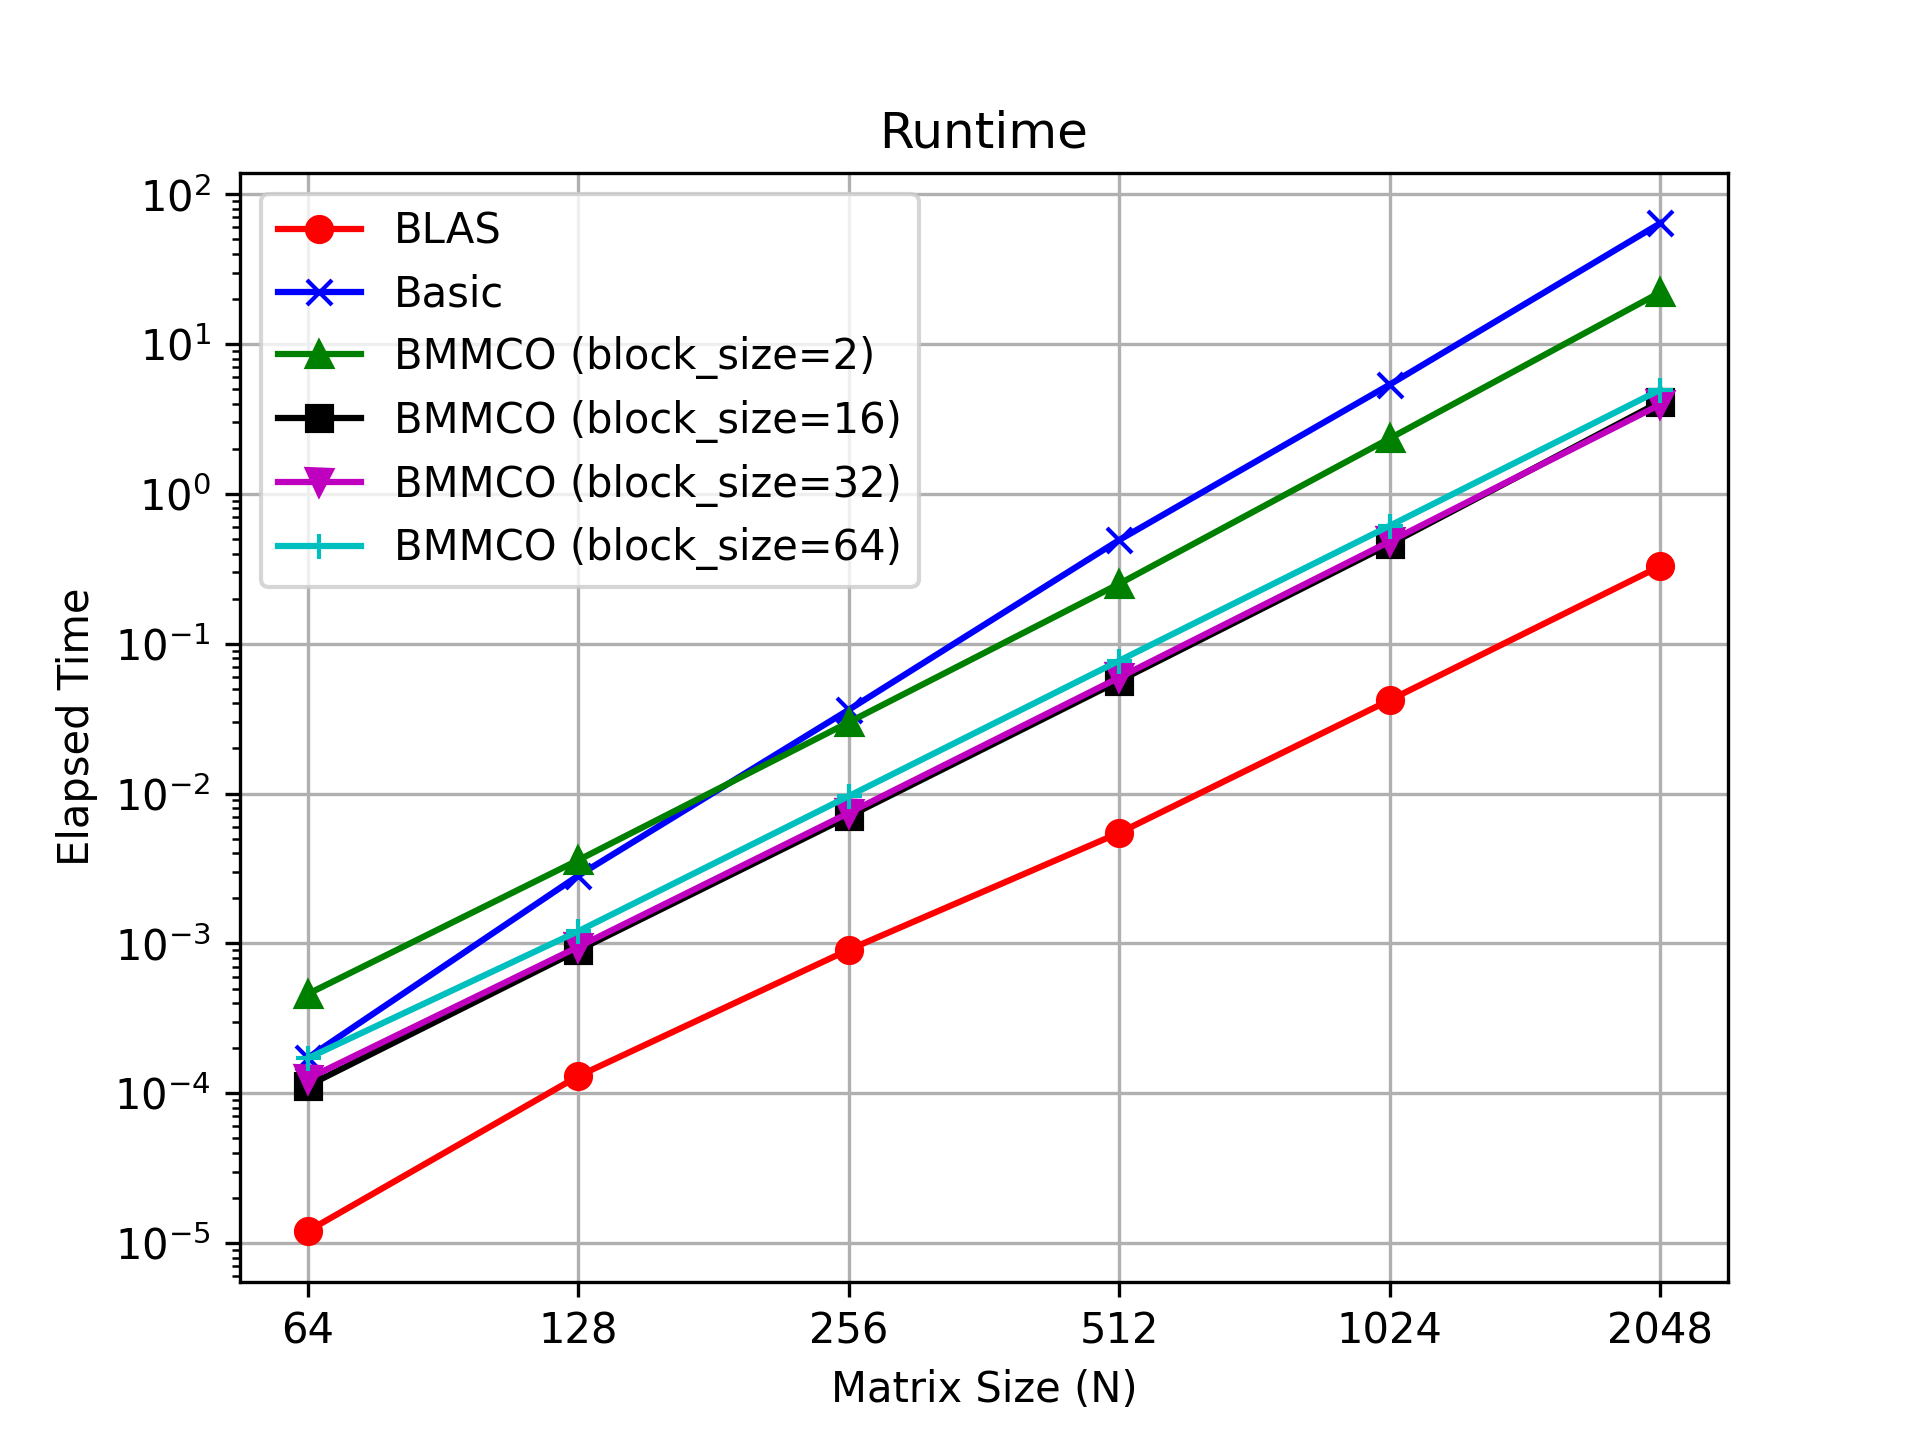
\includegraphics[width=1.0\linewidth]{images/Runtime.png}
%     \caption{Runtime comparison of all methods}
%     \label{fig:runtime}
% \end{figure}

\subsection{Comparison of Basic MM and CBLAS}
\label{subsec:basic-and-cblas}
\begin{comment}
    - Produce a chart comparing the performance of these two implementations across all problem sizes. The horizontal axis is problem size, the vertical axis is MFLOP/s (which you'll have to derive from runtime and your knowledge of the algorithm).
    - Discuss the performance of your Basic MM across the set of problem sizes. Do you see any changes of MFLOP/s across problem sizes? Describe the nature of those changes, if any, and provide an explanation of why the performance numbers change.
    - How does the performance of your Basic MM implementation compare to CBLAS, the reference implementation?
\end{comment}
% Describe the experiment in a few sentences: what question are you trying to answer, what problem sizes/etc did you use (it's ok to make reference back to Sec.~\ref{sec:methodology} so you don't have to repeat a lot of details. 

In this experiment, the objective is to establish a baseline for our evaluation by measuring the computational throughput (MFLOP/s) of Basic MM, an unoptimized implementation serving as our baseline, and CBLAS MM, a state-of-the-art, highly optimized implementation. The configuration details for this experiment are provided in Sec.~\ref{sec:methodology}.

As shown in Fig.~\ref{fig:mflops-Basic-CBLAS}, the MFLOP/s of the Basic MM decreases significantly as the problem size increases, while the MFLOP/s of the CBLAS implementation improves with larger matrix sizes. The decrease in Basic MM performance is almost inversely proportional to the matrix size, reflecting its inefficiency in terms of cache usage and memory access. In contrast, the CBLAS implementation shows a gradual improvement as the matrix size increases, with one exception: performance drops from \(64 \times 64\) to \(128 \times 128\). We believe this is caused by the initial discarded run for the \(64 \times 64\) problem size. It is likely that CBLAS’s \textit{cblas\_dgemm} method allocates an internal buffer based on the matrix size, which can be reused for efficiency in subsequent runs. The overhead of allocating this internal buffer is not negligible for smaller problem sizes, but the allocation process is skipped for \(64 \times 64\), leading to a performance drop for \(128 \times 128\).

Interestingly, the MFLOP/s of CBLAS sometimes exceeds the CPU core's theoretical peak performance of 39.2 GFLOP/s (see Sect.~\ref{sec:computeational-platform-and-software-environment}). During the execution, we verified that the program was not utilizing multiple cores by running the \textit{top} command, which showed a CPU usage value (\%CPU) close to, but less than, 100\%. We hypothesize that CBLAS is using advanced matrix multiplication techniques such as Strassen's algorithm, which can achieve a computational complexity better than \(O(N^3)\)\footnote{Strassen's algorithm has a complexity of approximately \(O(2^{2.8074})\).}. Therefore, our calculation of MFLOP/s using \(2N^3\) as \textit{ops} for CBLAS may not be entirely appropriate.

% Present the results of your experiment using either tabular forms of information, such as in Table~\ref{tab:MyTable1}, or using charts and graphs as in Fig.~\ref{fig:MyPlot1}.
\begin{figure}[htbp]
    \centering
    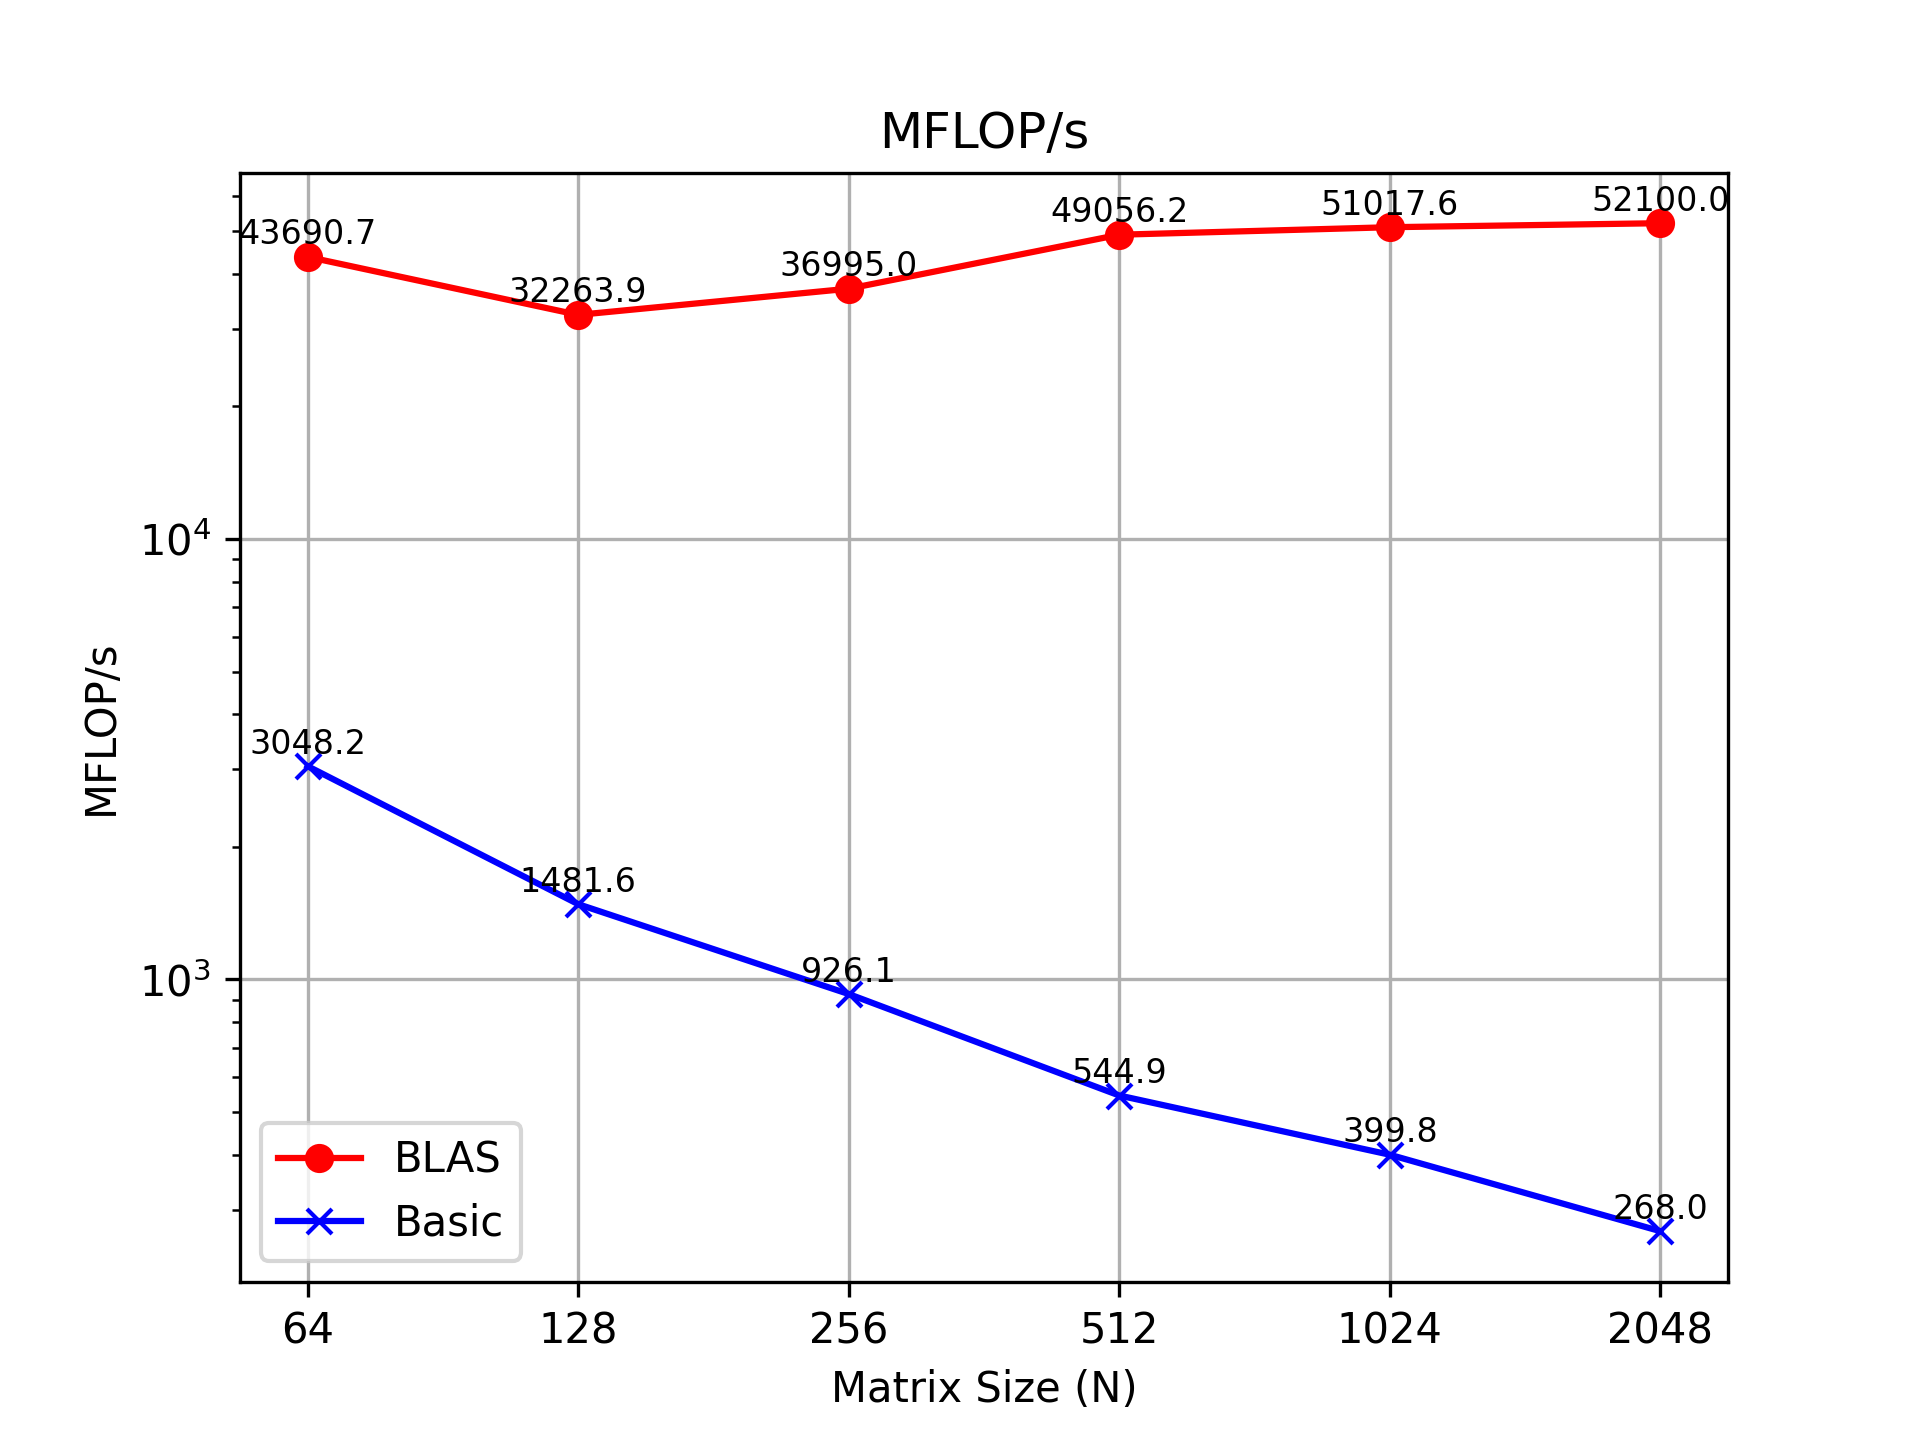
\includegraphics[width=1.0\linewidth]{images/Basic-MM-and-CBLAS_MFLOPs.png}
    \caption{\textbf{MFLOP/s comparison of Basic MM and CBLAS MM across different matrix sizes.} The matrix is \(N \times N\). Note that MFLOP/s decreases consistently on a logarithmic scale for Basic MM as the matrix size increases. In contrast, MFLOP/s gradually increases for CBLAS MM, with the exception of a performance drop from \(64 \times 64\) to \(128 \times 128\). This drop is likely due to the initial discarded run for the \(64 \times 64\) problem size.}
    \label{fig:mflops-Basic-CBLAS}
\end{figure}

\subsection{Blocked MM with Copy Optimization (BMMCO), and CBLAS}
\label{subsec:bmmco-and-cblas}

In this experiment, we evaluate the efficiency of the BMMCO implementation at four different block sizes by comparing its MFLOP/s with that of the CBLAS implementation. The configuration details for this experiment are provided in Sec.~\ref{sec:methodology}. Figure~\ref{fig:mflops-BMMCO-CBLAS} shows how block size and matrix size affect the MFLOP/s of BMMCO compared to the CBLAS MM implementation. From this figure, three key insights can be derived.

\begin{figure}[htbp]
    \centering
    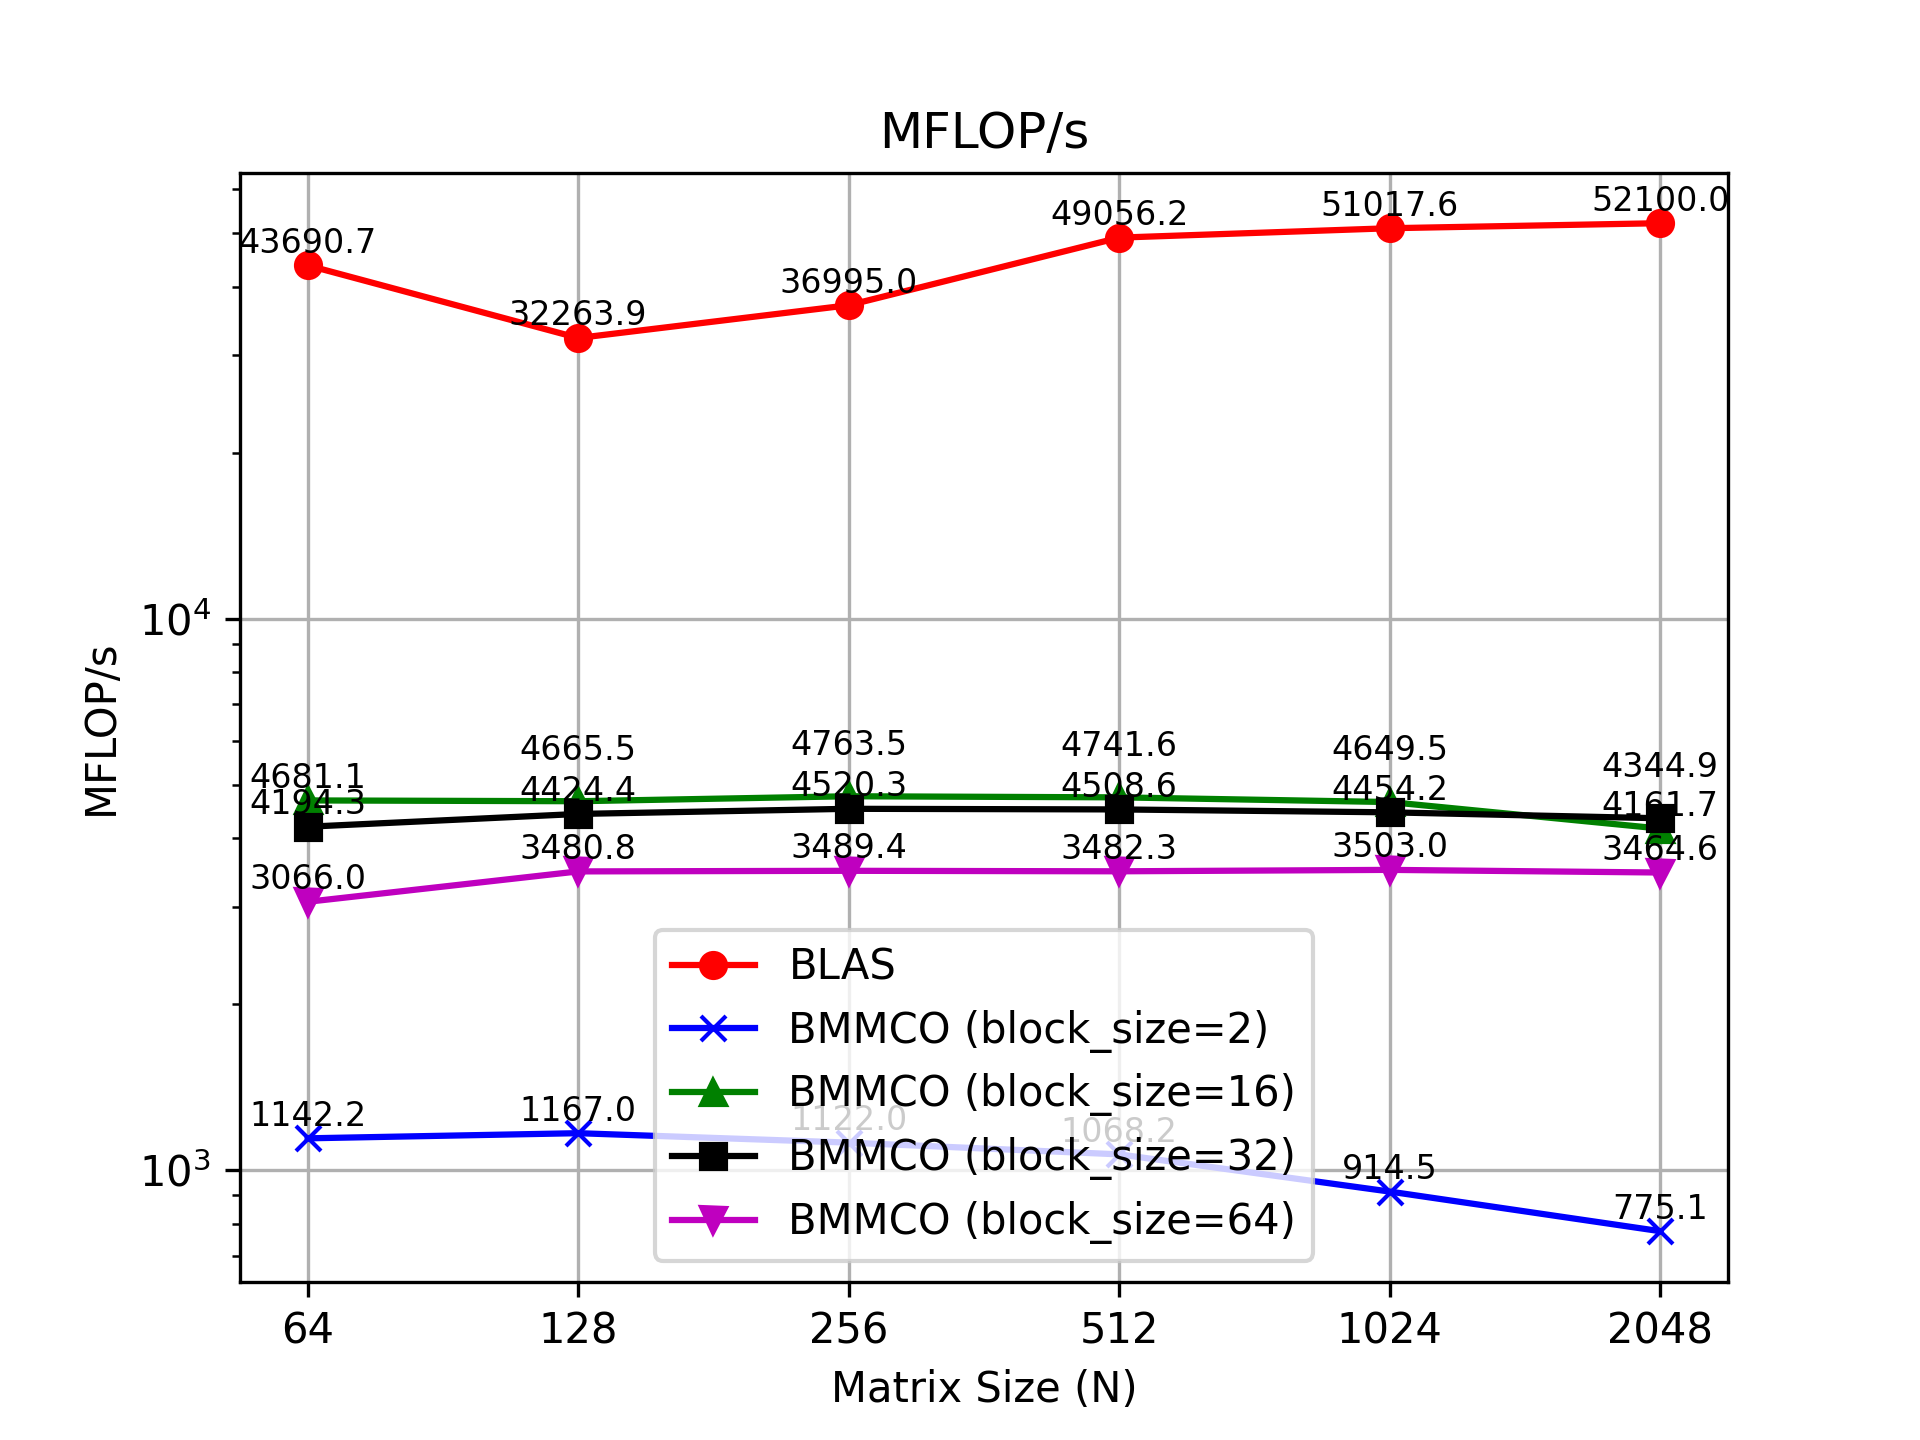
\includegraphics[width=1.0\linewidth]{images/BMMCO-and-CBLAS_MFLOPs.png}
    \caption{\textbf{MFLOP/s comparison of BMMCO and CBLAS MM across different block sizes and matrix sizes.} The matrix is \(N \times N\). The figure illustrates how BMMCO's performance varies with block sizes of 2, 16, 32, and 64, compared to the highly optimized CBLAS MM implementation. The block size of 2 is significantly inefficient due to the limited performance gain from small block sizes. While larger block sizes generally improve performance, the block size of 64 shows performance degradation due to exceeding the L1 cache capacity, as discussed in Sec.~\ref{subsubsec:l1-cache-fit}.}
    \label{fig:mflops-BMMCO-CBLAS}
\end{figure}

\subsubsection{Performance limitation of small block sizes}
\label{subsubsec:blocking-overhead}
The first insight is that the block size of 2 is significantly inefficient compared to larger block sizes, and its MFLOP/s decreases as the matrix size increases, following a similar trend to the Basic MM implementation in Section~\ref{subsec:basic-and-cblas}. This inefficiency is due to the fact that the performance gain is primarily limited by the small block size\footnote{The number of slow memory operations, \(m\), depends on the block size \(b\) and the matrix size \(N\). The total number of slow memory operations is proportional to \((2N_b + 2) \cdot N^2\), where \(N_b\) is the number of blocks. Compute intensity (CI), defined as \(CI = \frac{\textit{ops}}{\textit{number of slow memory accesses}}\), improves with larger block sizes as CI approaches \(n/N_b = b\) for large matrices.}.

\subsubsection{Impact of L1 cache capacity on performance}
\label{subsubsec:l1-cache-fit}
The second insight is that larger block sizes, particularly 16 and 32, perform better. The block size of 16 produced the best results, while the block size of 32 performed slightly worse. However, the block size of 64 showed a performance degradation of approximately 20-30\% compared to both 16 and 32. Initially, we expected larger block sizes to consistently provide better MFLOP/s, so these results were counterintuitive. This discrepancy is due to L1 cache utilization. As shown in Table~\ref{tab:memory-footprint-three-blocks-l1-cache}, the block size of 64 requires a memory footprint of 96 KiB for three blocks, which exceeds the 32 KiB L1 cache capacity (see Sec.~\ref{sec:computeational-platform-and-software-environment}). While block sizes up to \(32 \times 32\) fit within the L1 cache, the block size of 64 does not, resulting in performance degradation as tiling and blocking optimizations rely on fitting blocks into fast memory.

\begin{table}[htbp]
    \centering
    \begin{tabular}{c|c|c}
        \textbf{Block Size} & \textbf{3 Blocks (Bytes)} & \textbf{L1 Cache Fit} \\
        \hline
        \(2 \times 2\) & 96 B & Yes \\
        \(16 \times 16\)  & 6 KiB & Yes \\
        \(32 \times 32\)  & 24 KiB & Yes \\
        \(64 \times 64\)  & 96 KiB & No \\
    \end{tabular}
    \caption{\textbf{Memory footprint for different block sizes and L1 cache fit.} The table shows the memory required for three blocks of each size and whether they fit within the L1 cache (32 KiB). Block sizes up to \(32 \times 32\) fit, while \(64 \times 64\) does not.}
    \label{tab:memory-footprint-three-blocks-l1-cache}
\end{table}

\subsubsection{Remaining Performance Gap Between BMMCO and CBLAS}
\label{subsubsec:remaining-performance-gap-between-bmmco-cblas}
Even with the best BMMCO results (block size of 16), the CBLAS MM implementation still outperforms BMMCO by approximately tenfold. This significant performance gap suggests that there is still room for optimization, such as loop reordering, improved in-memory data layout strategies, and the use of advanced matrix multiplication algorithms like Strassen's algorithm.


\subsection{Findings and Discussion}
\label{subsec:findings-and-discussion}
\begin{comment}
    - Compare the differences between basic MM, blocked MM with copy: what differences and similarities do you see between the basic and blocked versions?
    - In places where one outperforms others, discuss why you believe that to be the case?  Does that correspond to any features of the hardware you are using?
    - Looking at all the datasets, do you see any changes of performance across problem sizes?
    - Describe the nature of those changes, if any, and provide an explanation of why the performance numbers change.
\end{comment}
From Figure\ref{fig:mflops-BMMCO-Basic}, we can gain two key insights.

\begin{figure}
    \centering
    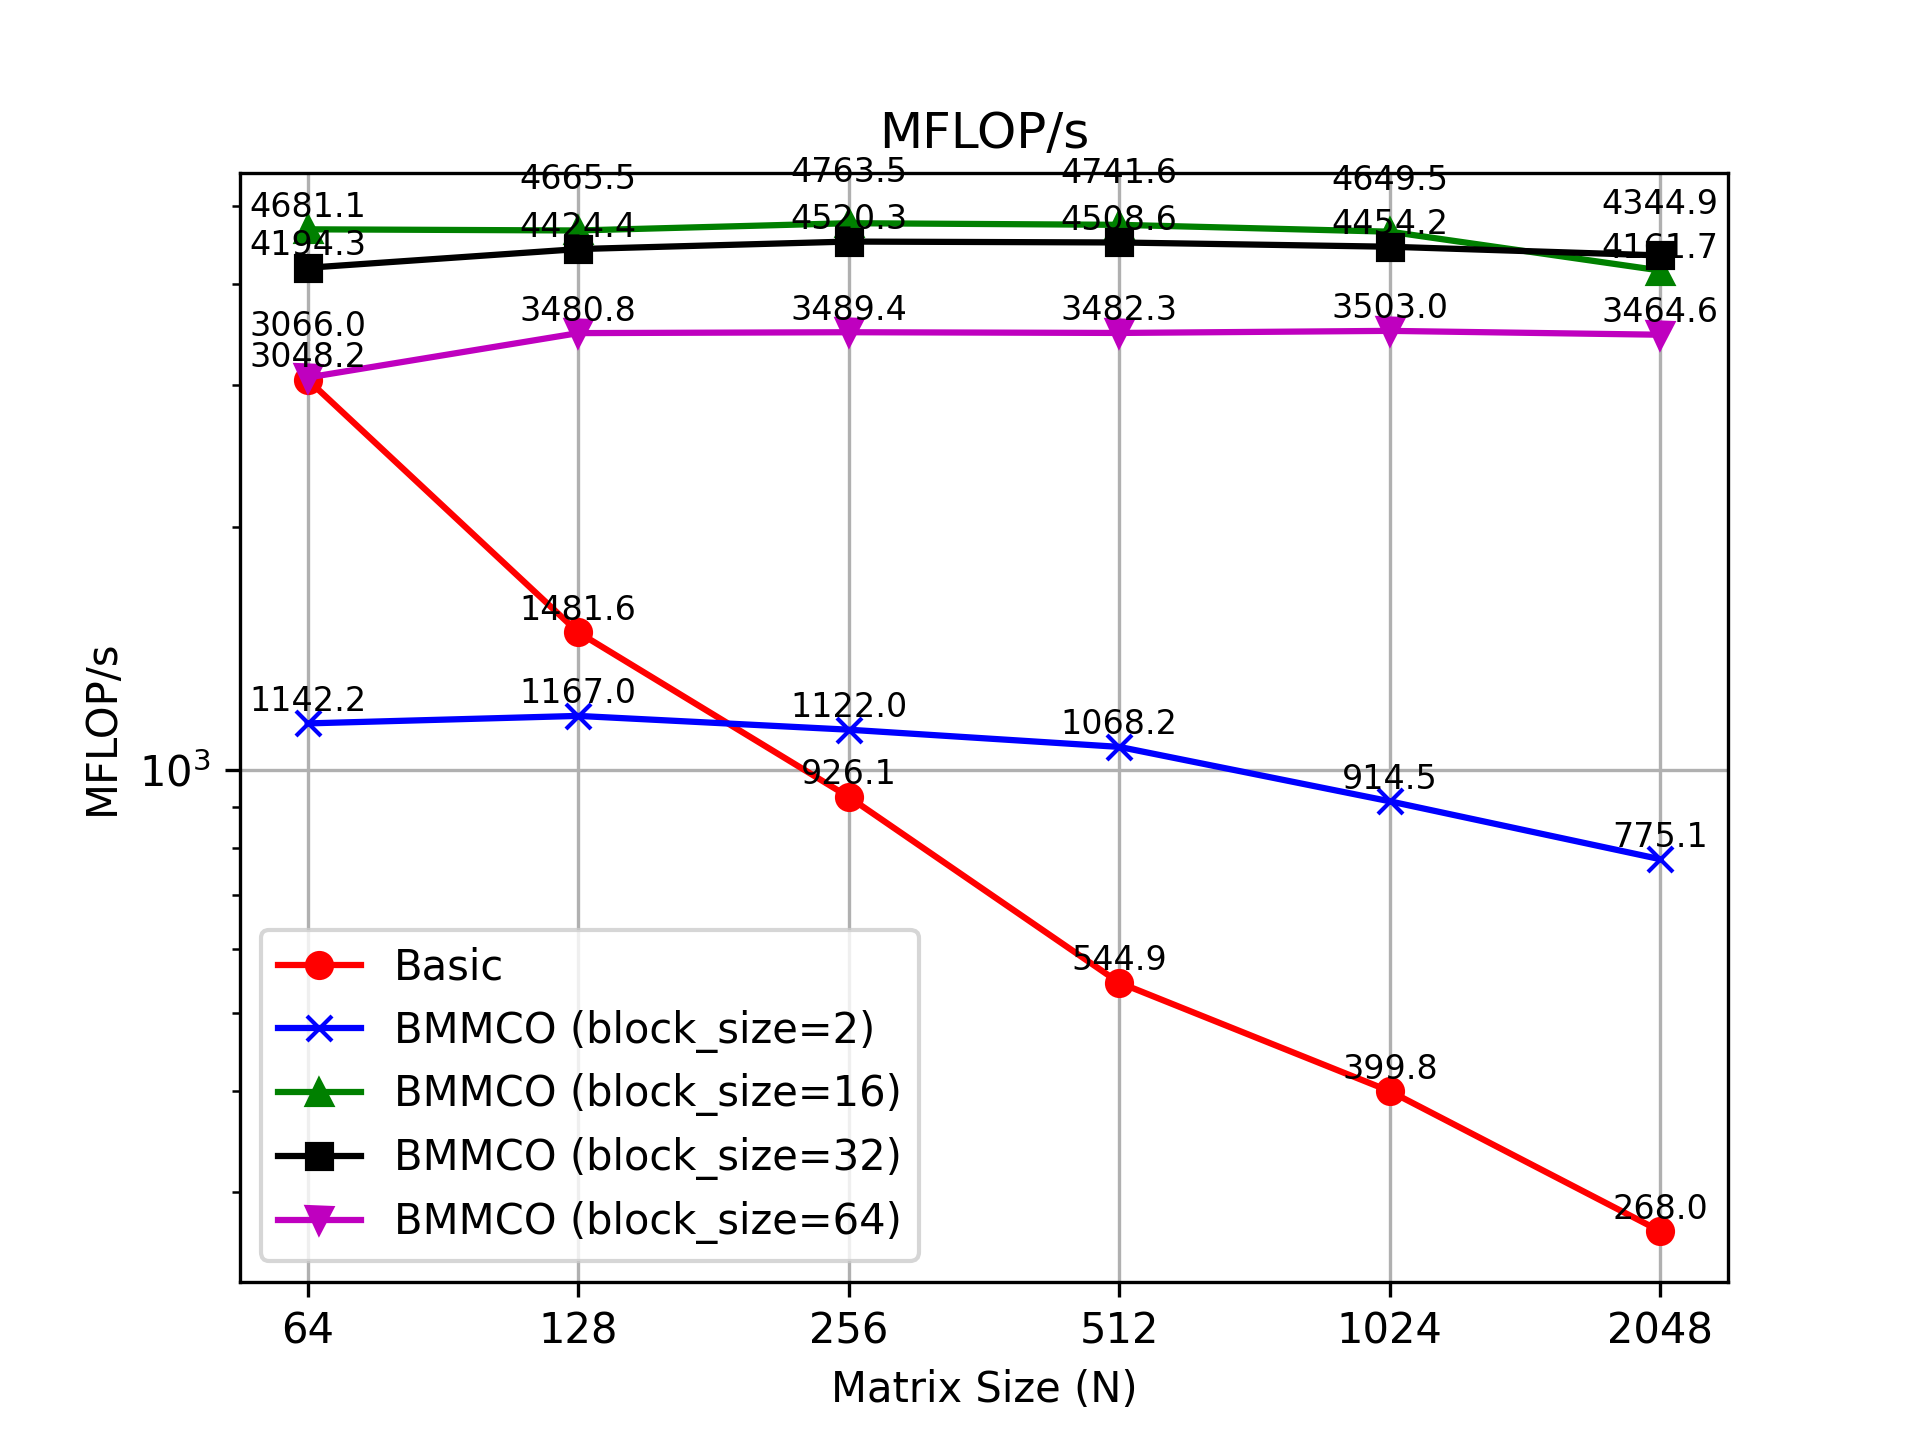
\includegraphics[width=1.0\linewidth]{images/BMMCO-and-Basic_MFLOPs.png}
    \caption{\textbf{MFLOP/s Comparison of BMMCO and Basic MM across Matrix Sizes.} This figure illustrates the performance differences between BMMCO and Basic MM across various matrix sizes. BMMCO shows more stable performance with larger matrix sizes due to optimization techniques such as blocking and copy, while Basic MM's performance degrades as the matrix size increases.}
    \label{fig:mflops-BMMCO-Basic}
\end{figure}

\FloatBarrier
\subsubsection{Poor performance of BMMCO with a block size of 2}
\label{subsubsec:poor-performance-bmmco-block-size-2}
The BMMCO implementation with a block size of 2 exhibits significantly lower performance than Basic MM for matrix sizes of \(64 \times 64\) and \(128 \times 128\). This can be attributed to the fact that matrices A, B, and C all fit entirely within the 512 KiB L2 cache, with a significant portion of them also fitting into the 32 KiB L1 cache for these sizes (see Table~\ref{tab:memory-footprint-three-matrices}). As a result, the benefits of blocking and copy optimization are outweighed by the overhead introduced (i.e., reading and writing blocks to internal buffer).

The MFLOP/s of BMMCO with a block size of 2 decreases as the problem size increases, following a similar trend observed in Basic MM, though the decline is more gradual. This is because, for larger matrix sizes that do not fit into the L2 cache, the overhead becomes relatively smaller, and the gains from optimization become more substantial.

\begin{table}[htbp]
    \centering\small
    \begin{tabular}{c|c|c|c|c}
        \textbf{Matrix Size} & \textbf{3 Matrices (Bytes)} & \textbf{L1} & \textbf{L2} & \textbf{L3} \\
        \hline
        \(64 \times 64\) & 96 KiB & No & Yes & Yes \\
        \(128 \times 128\) & 384 KiB & No & Yes & Yes \\
        \(256 \times 256\) & 1.5 MiB & No & No & Yes \\
        \(512 \times 512\) & 6 MiB & No & No & Yes \\
        \(1024 \times 1024\) & 24 MiB & No & No & Yes \\
        \(2048 \times 2048\) & 96 MiB & No & No & No \\
    \end{tabular}
    \caption{\textbf{Memory footprint for different matrix sizes and cache fit.} The table shows the memory footprint required to hold three matrices of varying sizes and whether they fit within the L1 cache (32 KiB), L2 cache (512 KiB), and L3 cache (32 MiB). Matrices up to \(128 \times 128\) fit in the L2 cache, and those up to \(512 \times 512\) fit within the L3 cache.}
    \label{tab:memory-footprint-three-matrices}
\end{table}

\subsubsection{Large Block Sizes Outperform Basic MM}
\label{large-block-outperform-basic}

For a matrix size of \(64 \times 64\), the performance of Basic MM is comparable to that of BMMCO with a block size of 64. This is because the matrix size and block size are equal, resulting in no significant performance gain from the BMMCO implementation.

However, BMMCO with larger block sizes consistently outperforms Basic MM, with performance remaining relatively stable across different matrix sizes, while Basic MM’s MFLOP/s decreases almost inversely as the matrix size increases. This improvement in BMMCO is due to performance gains that scale with the block size (see the footnote\footnotemark[3]) when the blocks fit into fast memory. In fact, the three blocks used in the optimization mostly fit within the L1 cache and fully fit within the L2 cache (see Table~\ref{tab:memory-footprint-three-blocks-l1-l2-cache}), allowing matrix multiplication to proceed with minimal slow memory access, thereby increasing efficiency.

In summary, without blocking and copy optimization, performance degrades significantly due to inefficient memory access. However, by leveraging these optimizations, both spatial and temporal locality are effectively utilized, leading to substantial improvements in overall efficiency.

\begin{table}[htbp]
    \centering
    \begin{tabular}{c|c|c|c}
    \textbf{Block Size} & \textbf{3 Blocks (Bytes)} & \textbf{L1 Cache} & \textbf{L2 Cache} \\
    \hline
    \(2 \times 2\) & 96 B & Yes & Yes \\
    \(16 \times 16\) & 6 KiB & Yes & Yes \\
    \(32 \times 32\) & 24 KiB & Yes & Yes \\
    \(64 \times 64\) & 96 KiB & No & Yes \\
    \end{tabular}
    \caption{\textbf{Memory Footprint for different block sizes  and L1 and L2 cache fit.} This table shows the memory footprint required to hold three blocks of different sizes and whether they fit within the L1 and L2 cache levels. Block sizes up to \(32 \times 32\) fit within the L1 cache, while larger block sizes fit within the L2 cache.}
    \label{tab:memory-footprint-three-blocks-l1-l2-cache}
\end{table}

% \begin{table}[htbp]
%     \centering
%     \begin{tabular}{c|c|c|c|c}
%     N & footprint & L1(32KB) & L2(512KB) & L3(32MB) \\
%     \hline
%     64 & 32KB & x & O & O \\
%     128 & 128KB & x & O & O \\
%     256 & 512KB & x & O & O \\
%     512 & 2MB & x & x & O \\
%     1024 & 8MB & x & x & O \\
%     2048 & 32MB & x & x & O \\
%     \end{tabular}
%     \caption{Memory footprint to hold single matrix}
%     \label{tab:memory-footprint-single-matrix}
% \end{table}

% Also, optionally include any additional insights you gained while doing these performance experiments.

% If this were an actual tech paper, here is where you would summarize the main findings and observations from the experiments: do the experiment results support your hypothesis? Sometimes the answer is a clear Y. Sometimes, the answer is Y for some circumstances, but not all, and it is important to spell this out.

% Sometimes, the experiments turn up unexpected negative results, and it is also important to point out those, as well. Science happens due to both successes and failures, and it is important to document failed experiments so that we can all learn from them.